\chapter{Wstęp}
\label{cha:pierwszyDokument}


Pierwsze obrazy wideo powstały już na początku XX wieku i opierały się na mechanicznie obracających się dyskach. Technologia ta istniała głownie w sferze badań akademickich i nie zdominowała rynku. Dopiero z wprowadzeniem cathode-ray tube (CRT), wraz z telewizją analogową, wideo zaczęło być wykorzystywane komercyjnie. Z czasem rozwój technologii pozwolił na wprowadzenie telewizji cyfrowej, która zapewniała wyższą jakość obrazu oraz lepsze wykorzystanie zasobów. Wideo razem z audio okazały się również znakomitym środkiem wymiany informacji. Coraz częściej wykorzystywane do komunikacji w czasie rzeczywistym zastępując tradycyjne połączenie telefoniczne w biznesie oraz dla zwykłych użytkowników. Również rozwój na rynku telefonów wspomógł powszechność wideo. W momencie kiedy praktycznie każdy aparat zaczął posiadać kamerę, wideo zaczęło konkurować ze zdjęciami jako metoda na utrwalenia danej chwili. Codziennie tak rejestrowane obrazy są przekazywane do rodziny, znajomych oddalonych o tysiące kilometrów. Kolejnym przykładem kiedy wideo zastępuje tradycyjne formy przekazu są blogi internetowe do tej pory prowadzone na zasadzie artykułów/postów, teraz zaczęły wykorzystywać wideo jako metodę przekazu informacji.

Dzięki coraz większym przepustowością i szerokiemu dostępu do Internetu w najnowszych czasach wykreował się jeszcze inny trend sprawiający że obrazy wideo są bardziej popularne. Mowa tu o platformach streamingowych takich jak - YouTube, Netflix czy HBOgo. Pozwalają one użytkownikom na oglądanie od krótkich filmików, przez seriale, po pełnometrażowe filmy nawet w rozdzielczościach 4k. Przewidywane jest, że do 2022, aż 82 procent całego ruchu IP, to będzie wideo \cite{prediction}. \par

%.Jako kolejny kierunek rozwoju wideo można potraktować powstałe w ostatnich latach platformy, typu Youtube, netflix czy HBOgo, pozwalające użytkownikom na streamowanie od krótkich %filmików, przez seriale, po pełnometrażowe filmy nawet w rozdzielczościach 4k. \par

Wszystkie wymienione wyżej aspekty sprawiły, że wideo stało się codziennością w życiu większości ludzi.\par

Na obecnym etapie rozwoju technologii, oczekiwania odbiorcy co do jakości otrzymywanego wideo znacznie wzrosły. Na drugiej szali pozostają ograniczenia dotyczące medium i optymalnego wykorzystania zasobów po stronie klienta i serwera. Odnosząc się do powyższego istotną kwestią staje się monitorowanie jakości transmitowanego wideo i dostosowywanie go do potrzeb użytkownika. Jednak problem w ocenie jakości wideo jest tu o tyle trudny, że dotychczas najbardziej wiarygodnym wskaźnikiem jest tu opinia ludzka, nie powiązana(?żadnym agorytmem?) z technicznymi aspektami ?obrazu?\todo{, ciężka do powiązania technicznymi cechami wideo}. W niniejszej Pracy zostanie przedstawiony algorytm pozwalający na bardziej zautomatyzowaną ocenę jakości wideo w oparciu o metryki full-reference (FR) i no-reference (NR) oraz zaprezentowana zostanie wykorzystana metodologia badań.



\chapter{Wprowadzenie teorytyczne}
\label{cha:pierwszyDokument}

W niniejszym rozdziale przedstawiono najważniejsze zagadnienia dla przeprowadzonych badań. Opisane one zostały w sposób pozwalający czytelnikowi na odpowiednie zrozumienie dalszej częci pacy, pomijając niezwiązane szczegóły. Pierwsza część rozdziału dotyczy tematu wideo. Przedstawiono jego definicję, oraz wybrane cechy statystyczne biorące udział w trakcie badań .W kolejnej części przedstawiono zagadnienia z obszaru uczenia maszynowego. Wyjaśniona została jej ogólna koncepcja, a następnie opisano użyte algorytmy.


\section{Wideo}

<definicja ciężko znaleźć :( >
Wideo jest formą elektronicznego zapisu sygnału wizji (analogowego bądź cyfrowego). W swojej surowej postaci jest to sekwencja pojedynczych ramek. Takie pliki zajmują bardzo dużo przestrzeni dyskowej. Przykładowo obraz o rozdzielczości 1920x1080 z 24 ramkami na sekundę o długości 30 sekund zajmuje ponad \todo{sprawdzić ile dokładnie}20 GB w pamięci komputera. Tak duże rozmiary znacząco ograniczają możliwości przechowywania i transmisji dla zwykłych użytkowników. Dlatego praktycznie każdy plik wideo wykorzystuje kodeki, czyli pewne ustandaryzowane zasady kompresji/dekompresji. Do najpopularniejszych należą H.265 i H.264 powszechnie używany w Internecie do transmitowania multimediów \cite{video_codecs}. Błędy podczas tego procesu mogą powodować powstanie zakłóceń w odtwarzanym obrazie. Aby mierzyć poziom uszkodzeń oraz monitorować stan wideo badacze zdefiniowali wiele metryk.\par.

\section{Metryki}
%https://books.google.se/books?id=JbtPCwAAQBAJ&pg=PA32&dq=video++quality+metrics+full+reference&hl=en&sa=X&ved=0ahUKEwi4wtGc2YfiAhWx-ioKHZJtAtcQ6AEIKjAA#v=onepage&q=video%20%20quality%20metrics%20full%20reference&f=false

Jakość danego wideo jest najtrafniej oceniona dzięki tak zwanej ocenie subiektywnej. Polega ona na określeniu jakości odbioru przez człowieka na podstawie jego odczuć. Niestety aby takie badanie było miarodajne należy je przeprowadzić w odpowiednich warunkach, przygotować zestaw testów, zrekrutować uczestników oraz cały czas nadzorować jego przebieg. Wszystko to generuje duże koszta i zabiera cenny czas, ale przede wszystkim nie pozwala na ocenę jakości w czasie rzeczywistym na przykład podczas streamowania video. Problem ten rozwiązują metryki jakości wideo. które w przeciwieństwie do oceny subiektywnej, bazują na obiektywnych pomiarach właściwości\cite{vqm}.\par
Metryki video mogą zostać sklasyfikowane na podstawie tego czy do ich policzenia wymagana jest obecność niezakłóconego pliku video. Metryki, które wymagają takiego pliku określane są mianem {\em ang. full-reference} (FR). Porównują one właściwości zakłóconego i nie zakłóconego video, aby na podstawie tak otrzymanych informacji dokonać estymaty jakości. Innym rodzajem metryk są metryki {\em ang. no-reference} (NR). Dokonują one oceny jakości na podstawię zniekształconego video i nie wymagają do tego żadnych dodatkowych informacji\cite{vqm}.\par

Poniżej zostały przedstawione wskaźniki jakości typu NR.

%\let\labelitemi\labelitemii
\begin{itemize}[label=$\bullet$]
\item Blokowosć({\em ang. Blockiness}) -- powstaje podczas procesu kwantyzacji bloków pikseli i objawia się poprzez zauważalną granice między tymi blokami\cite{blockiness}. W niniejszej pracy została przyjęta skala 0-3570. Im większa wartoć, tym mniej widoczne zakłócenie. Dla obrazu bez zakłóceń około 0.9-1.01\cite{agh_vqm}
\begin{figure}[h]
\centerline{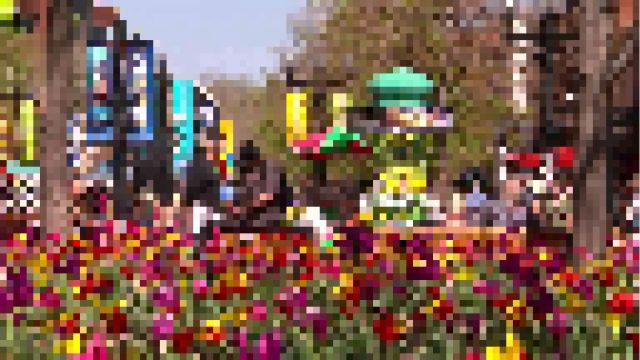
\includegraphics[scale=0.5]{blockiness}}
\caption{Przykładowy obraz z zakłóceniami spowodowanymi blokowoscią\cite{agh_vqm}}
\label{fig:xccs}
\end{figure}

\item spatialact
\item letterbox 
\item pillarbox 
\item blockloss 
\item blur(rozmaranie) 
\item temporalac
\item blockout 
\item freezing 
\item exposure 
\item contrast 
\item brightness
\item interlace 
\item noise 
\item slice 
\item flickering
\end{itemize}

metryki FR i ich wymienienie w oparciu o https://ieeexplore.ieee.org/document/5506331

\begin{itemize}[label=$\bullet$]
\item SSIM
\item VMAF
\item PSNR
\item itp
\end{itemize}

pozostałe cehcy wideo: 

\begin{itemize}[label=$\bullet$]
\item Rozdzielczoć -- miara określająca rozmiar ramki. Jednostką są pixele. Podawana jest zazwyczaj w następujący sposób: szerokość x wysokość. Do badań zostały użyto wideo o rozdzielczościach: 3840x2160, 1920x1080, 704x576, 640x480, 352x288. 
\item Klatki na sekundę( ang.frames per second, fps ) -- liczba ramek wyświetlonych w czasie sekundy. W telewizji jest to 25 ramek na sekundę. Do badań użyto: 60, 30, 25, 24 fps
\end{itemize}

\section{Algorytmy uczenia maszynowego }
\label{cha:pierwszyDokument}

\begin{itemize}
\item Ogólne informacje uczeniu maszynowym/
\item Przedstawienie wybranych algorytmów 
\end{itemize}

\chapter{Metodologia badań}
\label{cha:pierwszyDokument}

\section{Dane}
\label{cha:pierwszyDokument}

\begin{itemize}
\item Wybrane narzędzia
\item Opis zebranych danych
\item Przedstawienie data flow(pobieranie-> czyszczenie->normalizacja->przygotowanie formatu dla modeli).
\item Wizualizacja danych
\end{itemize}


\section{Modele }
\label{cha:pierwszyDokument}

\begin{itemize}
\item Opis zastosowanych paramtrów/technik podczas trenowania.
\item Przedstawienie wyników 
\end{itemize}


\chapter{Analiza i wnioski }
\label{cha:pierwszyDokument}

\begin{itemize}
\item Interpretacja wyników
\item Opis innych czynników mogących zaburzyć ich prawdziwoć
\item Co nie zostało uwzględnione 
\end{itemize}


\chapter{Podsumowanie}
\label{cha:pierwszyDokument}

\begin{itemize}
\item Czy cel pracy został osiągniety.
\item Możliwoci rozbudowy
\end{itemize}





